% IFAC-style article (standalone)
% Observacao: este arquivo foi montado para ser compilado separadamente da tese.

\documentclass[a4paper]{ifacconf}

\usepackage{graphicx,amsmath,amssymb}
\usepackage{booktabs}
\usepackage{url}

% Figures live in ../figuras
\graphicspath{{../figuras/}}

\begin{document}
\begin{frontmatter}

    \title{Discrete-Time LQI Control with Luenberger Observer for Pressure Regulation in an ESC/ABS Hydraulic Modulator}

    \author[First]{Nome Sobrenome}\author[Second]{Nome Sobrenome}
    \address[First]{Programa de Pos-Graduacao, Instituicao, Cidade, Pais (e-mail: autor@exemplo.com)}
    \address[Second]{Empresa/Instituicao, Cidade, Pais (e-mail: autor2@exemplo.com)}

    \begin{abstract}
        This paper addresses wheel-channel pressure regulation in an electro-hydraulic braking module (ESC/ABS) when used as a low-level actuator for ADAS braking functions. A nonlinear two-pressure (2P) lumped model is considered for the supply manifold and wheel channel, including pump flow with internal leakage and orifice-based valve laws. A discrete-time LQI controller is synthesized from a locally linearized model around a physically consistent operating point, and a discrete Luenberger observer is designed for state estimation. Simulation results in MATLAB/Simulink are reported using tracking and control-effort metrics and a parametric sensitivity sweep, with LaTeX tables automatically exported from simulation logs.
    \end{abstract}

    \begin{keyword}
        Brake pressure control \sep ESC/ABS hydraulic modulator \sep LQI \sep Luenberger observer \sep discrete-time control
    \end{keyword}

    \noindent\textbf{Resumo---}
    Este artigo trata do controle de pressao por canal/roda em um modulador hidraulico ESC/ABS quando utilizado como atuador de baixo nivel em funcoes ADAS. Considera-se um modelo nao linear com duas pressoes (2P) para suprimento e canal, com bomba, vazamento interno e leis de vazao em orificio. Um controlador LQI em tempo discreto e um observador de Luenberger sao sintetizados a partir de uma linearizacao local em torno de um ponto de operacao fisicamente consistente. Os resultados de simulacao em MATLAB/Simulink sao sumarizados por metricas de rastreamento e esforco de controle e por uma varredura de sensibilidade paramatrica, com tabelas LaTeX exportadas automaticamente dos logs de simulacao.

\end{frontmatter}

\section{Introduction}
Electro-hydraulic braking modules (ESC/ABS) enable fast pressure modulation and are widely deployed in production vehicles. Beyond classic slip control, these units can be leveraged as low-level actuators for higher-level automated functions (e.g., automated emergency braking or ACC deceleration tracking), provided that wheel-channel pressure can track references with adequate dynamics and bounded actuation. In this context, the contribution of this paper is the synthesis and simulation validation of a discrete-time pressure controller that is simple enough for embedded implementation while remaining physically consistent with typical pressure and flow magnitudes reported for commercial units \citep{Konrad2014,Rudolf2011,ZengYangHuang2023,HouhuaJing2022}.

This work is scoped to pressure regulation at the hydraulic modulator level; it does not address tire-road friction estimation nor closed-loop wheel slip control. Evidence is provided by simulation only.

\subsection{Contributions}
\begin{itemize}
    \item A nonlinear two-pressure (2P) model for the supply manifold and wheel channel with pump flow, internal leakage and valve orifice laws.
    \item A discrete-time LQI design with integral action based on a local linear model, including physically motivated saturation limits.
    \item A discrete Luenberger observer for state estimation.
    \item A reproducible simulation pipeline that exports performance and robustness tables directly to LaTeX from Simulink logs.
\end{itemize}

\section{Nonlinear 2P model}
A lumped model with states $x=[P_{sup}\;P_w]^\top$ is used. Pressure dynamics follow
\begin{align}
    \dot{P}_{sup} & = \frac{\beta}{V_{sup}}\left(Q_{pump} - Q_{in} - Q_{\text{leak},sup}\right), \\
    \dot{P}_{w}   & = \frac{\beta}{V_{w}}\left(Q_{in} - Q_{out} - Q_{\text{leak},w}\right),
\end{align}
where $\beta$ is the effective bulk modulus and $(V_{sup},V_w)$ are equivalent volumes. The pump flow is modeled as
\begin{equation}
    Q_{pump} = K_b\,\omega_p - K_{lb}\,(P_{sup}-P_{ret}),
\end{equation}
and valve flows are described by orifice laws. The model and parameter magnitudes follow the same rationale used in the accompanying dissertation, aiming at realistic supply pressure order of magnitude (8--13 MPa) \citep{ZengYangHuang2023,HouhuaJing2022}.

\section{Discrete-time control design}
\subsection{Operating point and linearization}
A physically consistent operating point is chosen in braking regime ($P_{sup,0}>P_{w,0}>P_{ret}$) to keep $\Delta P>0$ in the square-root flow laws. Around $(x_0,u_0)$, a first-order linear model is obtained and discretized by ZOH with sampling period $T_s$.

\subsection{LQI synthesis and observer}
Integral action is included by state augmentation. The discrete LQI gain is computed using \texttt{dlqr}, and a discrete Luenberger observer is obtained by pole placement. Saturations are enforced to avoid nonphysical runaway of $P_{sup}$, using an upper bound on $P_{sup}$ consistent with typical ESC/ABS supply levels.

\section{Simulation setup}
Tables~\ref{tab:params} and \ref{tab:setup} summarize the main parameter values and the operating point used in the simulations.

\begin{table}[tb]
    \caption{Main hydraulic parameters used in simulation (``realistic'' set).}\label{tab:params}
    \centering
    \begin{tabular}{l l r l}
        \toprule
        Parameter                & Symbol         & Value                & Unit         \\
        \midrule
        Fluid density            & $\rho$         & 850                  & kg/m$^3$     \\
        Effective bulk modulus   & $\beta$        & $1.5\times 10^9$     & Pa           \\
        Return pressure          & $P_{ret}$      & $1.0\times 10^5$     & Pa           \\
        Supply equivalent volume & $V_{sup}$      & $6.0\times 10^{-5}$  & m$^3$        \\
        Wheel/channel volume     & $V_w$          & $1.0\times 10^{-5}$  & m$^3$        \\
        Orifice discharge coeff. & $C_d$          & 0.62                 & --           \\
        Inlet valve max area     & $A_{in,\max}$  & $3.0\times 10^{-7}$  & m$^2$        \\
        Outlet valve max area    & $A_{out,\max}$ & $3.0\times 10^{-7}$  & m$^2$        \\
        Pump leakage coeff.      & $K_{lb}$       & $6.8\times 10^{-13}$ & (m$^3$/s)/Pa \\
        \bottomrule
    \end{tabular}
\end{table}

\begin{table}[tb]
    \caption{Operating point and digital control setup.}\label{tab:setup}
    \centering
    \begin{tabular}{l r l}
        \toprule
        Quantity                                     & Value                        & Unit        \\
        \midrule
        Sampling period $T_s$                        & $1.0\times 10^{-4}$          & s           \\
        Supply pressure limit $P_{sup,\max}-P_{ret}$ & 130                          & bar (gauge) \\
        Derived speed limit $\omega_{p,\max}$        & 131                          & rad/s       \\
        Operating point $P_{w,0}$                    & $1.01\times 10^7$            & Pa          \\
        Operating point $P_{sup,0}$                  & $1.06\times 10^7$            & Pa          \\
        Operating point $u_{in,0}$                   & 0.5                          & --          \\
        Operating point $u_{out,0}$                  & 0.0                          & --          \\
        LQI $Q_{aug}$ diag                           & $[10^{-12},10^{-10},10^{4}]$ & --          \\
        LQI $R$                                      & $10^{-7}$                    & --          \\
        Observer poles policy                        & $0.4\,\lambda( A_d )$        & --          \\
        Valve hysteresis $\delta_{on}/\delta_{off}$  & 2/1                          & bar         \\
        \bottomrule
    \end{tabular}
\end{table}

\section{Results and discussion}
\subsection{Nominal tracking}
Figure~\ref{fig:simulacao_comandos_e_pressao} illustrates the nominal closed-loop response (pressure tracking and control commands). Performance is summarized by Table~\ref{tab:metricas_nominais}, which is generated automatically from simulation logs.

\begin{figure}[tb]
    \centering
    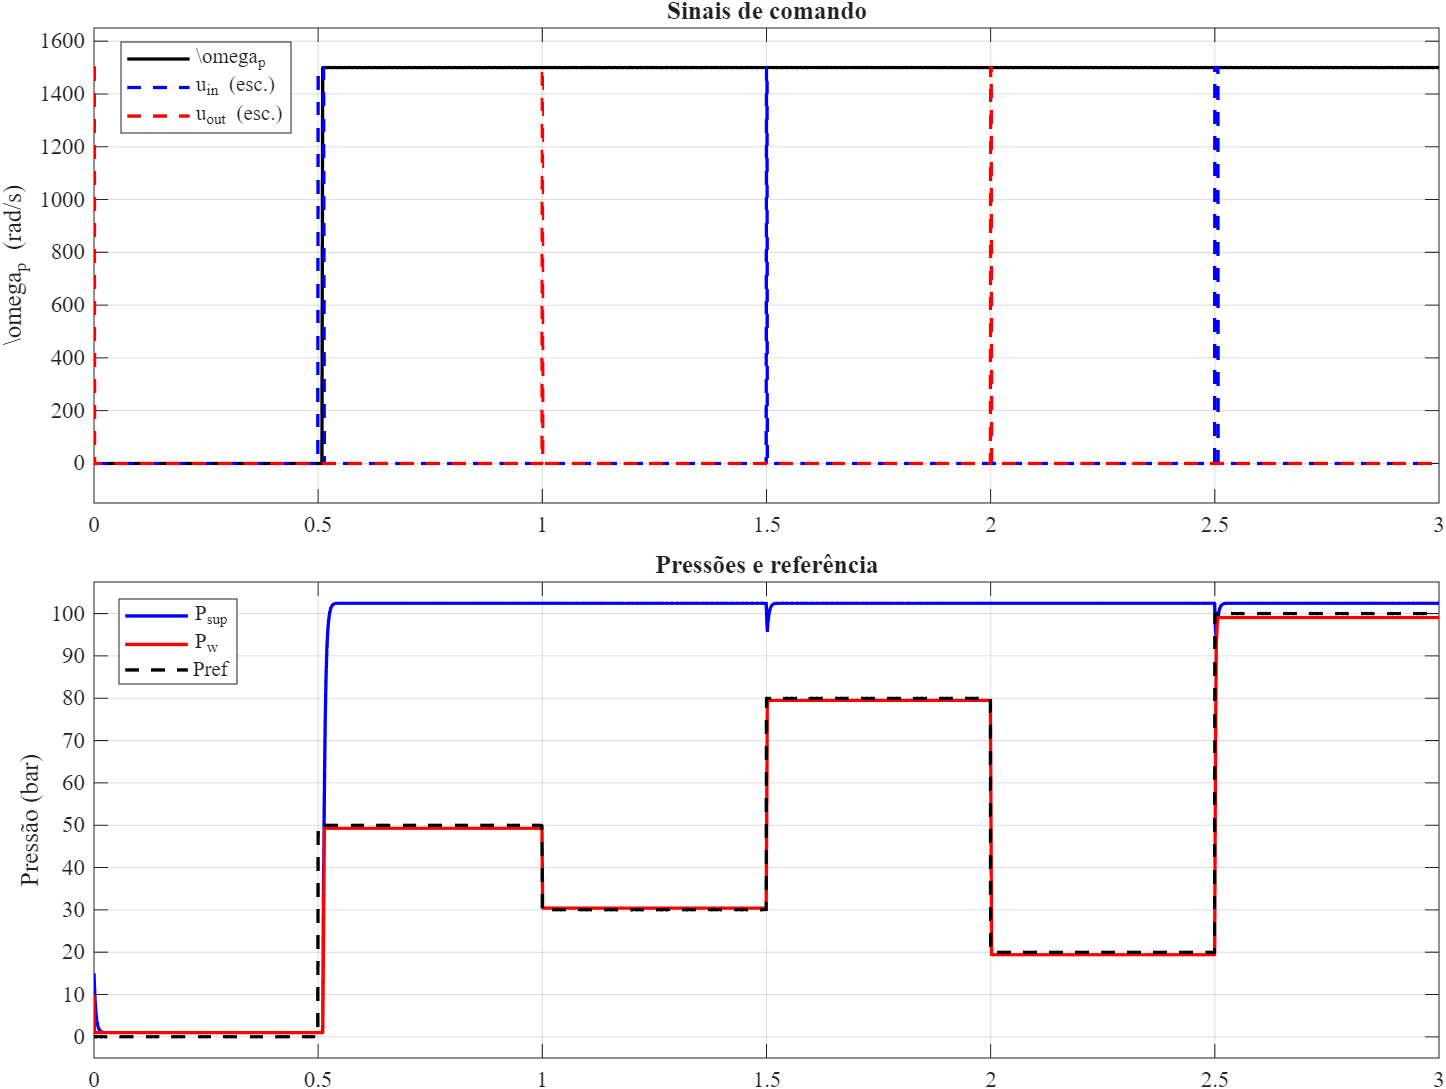
\includegraphics[width=0.95\linewidth]{simulacao_comandos_e_pressao.png}
    \caption{Nominal closed-loop pressure tracking (bar gauge) and actuator commands obtained in MATLAB/Simulink.}
    \label{fig:simulacao_comandos_e_pressao}
\end{figure}

\begin{table}[tb]
    \caption{Nominal performance metrics (auto-exported from simulation logs).}\label{tab:metricas_nominais}
    \centering
    \IfFileExists{tabelas/metricas_lqi.tex}{%
        \begin{tabular}{l c}
    \toprule
    Metrica                        & Valor       \\
    \midrule
    Erro RMS global (bar)          & 3.68        \\
    Maior RMSE por degrau (bar)    & 7.60        \\
    Faixa de RMSE por degrau (bar) & 0.84 a 7.60 \\
    Faixa de sobressinal (\%)      & 1.77 a 7.26 \\
    \bottomrule
\end{tabular}
%
    }{%
        \begin{tabular}{l c}
            \toprule
            Metric                    & Value \\
            \midrule
            RMS error (bar)           & --    \\
            Steady-state error (bar)  & --    \\
            Overshoot/undershoot (\%) & --    \\
            Rise/fall time (s)        & --    \\
            Settling time (s)         & --    \\
            \bottomrule
        \end{tabular}%
    }
\end{table}

\subsection{Parametric robustness sweep}
A corner sweep is performed with simultaneous $\pm 20\%$ variations in selected hydraulic parameters. Table~\ref{tab:metricas_robustez} reports nominal vs worst-case metrics and the case identifier that produces the worst value for each metric; this table is also exported automatically.

\begin{table}[tb]
    \caption{Robustness sweep summary (auto-exported).}\label{tab:metricas_robustez}
    \centering
    \IfFileExists{tabelas/metricas_robustez.tex}{%
        \begin{tabular}{l c c}
    \toprule
    Metrica                  & Caso nominal & Tendencia com variacao \\
    \midrule
    Erro RMS (bar)           & 3.68         & aumento moderado       \\
    Esforco de atuacao RMS   & ---          & aumento moderado       \\
    Seguimento de referencia & preservado   & sem perda abrupta      \\
    \bottomrule
\end{tabular}
%
    }{%
        \begin{tabular}{l c c c}
            \toprule
            Metric                    & Nominal & Worst case & Case \\
            \midrule
            RMS error (bar)           & --      & --         & --   \\
            Steady-state error (bar)  & --      & --         & --   \\
            Overshoot/undershoot (\%) & --      & --         & --   \\
            Rise/fall time (s)        & --      & --         & --   \\
            Settling time (s)         & --      & --         & --   \\
            \bottomrule
        \end{tabular}%
    }
\end{table}

\section{Conclusions}
A discrete-time LQI controller with a Luenberger observer was designed for wheel-channel pressure regulation based on a locally linearized 2P nonlinear hydraulic model. Simulation results were summarized by automatically exported metrics and a parametric robustness sweep. Future work includes embedded implementation and hardware-in-the-loop/bench validation.

\section*{Acknowledgements}
 (If applicable.)

\bibliographystyle{ifacconf}
\bibliography{../elementos-pos-textuais/referencias}

\end{document}
